\section{Evaluation}

We have performed a full system implementation on a Xilinx ZCU102 development board, featuring a Xilinx Zynq UlraScale+ XCZU9EG SoC. For this work, we utilize a combination of synthetic and real benchmarks. Our synthetic benchmark.
\todo[inline]{
  Talk about IO intensive and memory intensive benchmarks to be designed....
  We also include a study of the behavior of real applications from the San Diego Vision Benchmark Suite (SD-VBS) \cite{SD-VBS}, which comes with multiple input sizes....
}
\todo[inline]{
    DH: Maybe we could use AES from MiBench ?
}

As mentioned earlier, the high-performance master ports, namely HPMs, serve as a gateway from the PS to the PL. We implemented our scheduler IP, SchIM, responding under the physical addresses of HPM0 right after the PS. By doing so, any transaction toward the PL has to go through the SchIM. Hence, all memory requests yield to the scheduling policy being enforced by the scheduler. Design features of SchIM implementation and configuration interface are detailed in section ??.


At the preprocessing stages, an AXI Performance Monitor (APM) unit connected to the bus interface between the HPM0 and the scheduler. It is crucial to affirm that this medium does not affect the transaction flow toward the PL.  APMs are powerful tools available in the PS and instantiable in the PL capable of measuring primary performance metrics (for AXI4, AXI4-Lite, or AXI4-Stream-based systems) such as bus latency for specific master/slave or amount of memory traffic for the particular duration. Moreover, APM offers the functionality of logging the necessary information about data transfers between any master and slave communicating in the AXI protocol. In this work, we program APMs to profile the behavior of the benchmarks to analyze the task's deadline. SchIM employs profiled information on task deadlines to make scheduling decisions (e.g., enforce EDF policy) for hard real-time jobs.

  \subsection{Performance degradation}
  
  \subsection{Platform Capabilities}
    Here, discuss Fig.\ref{fig:bandwidth_comparison}
    \todo[inline]{Broad evaluation of the bandwidth offer by the ZCU102 depending on the route considered.}
    \begin{figure}
      \centering
      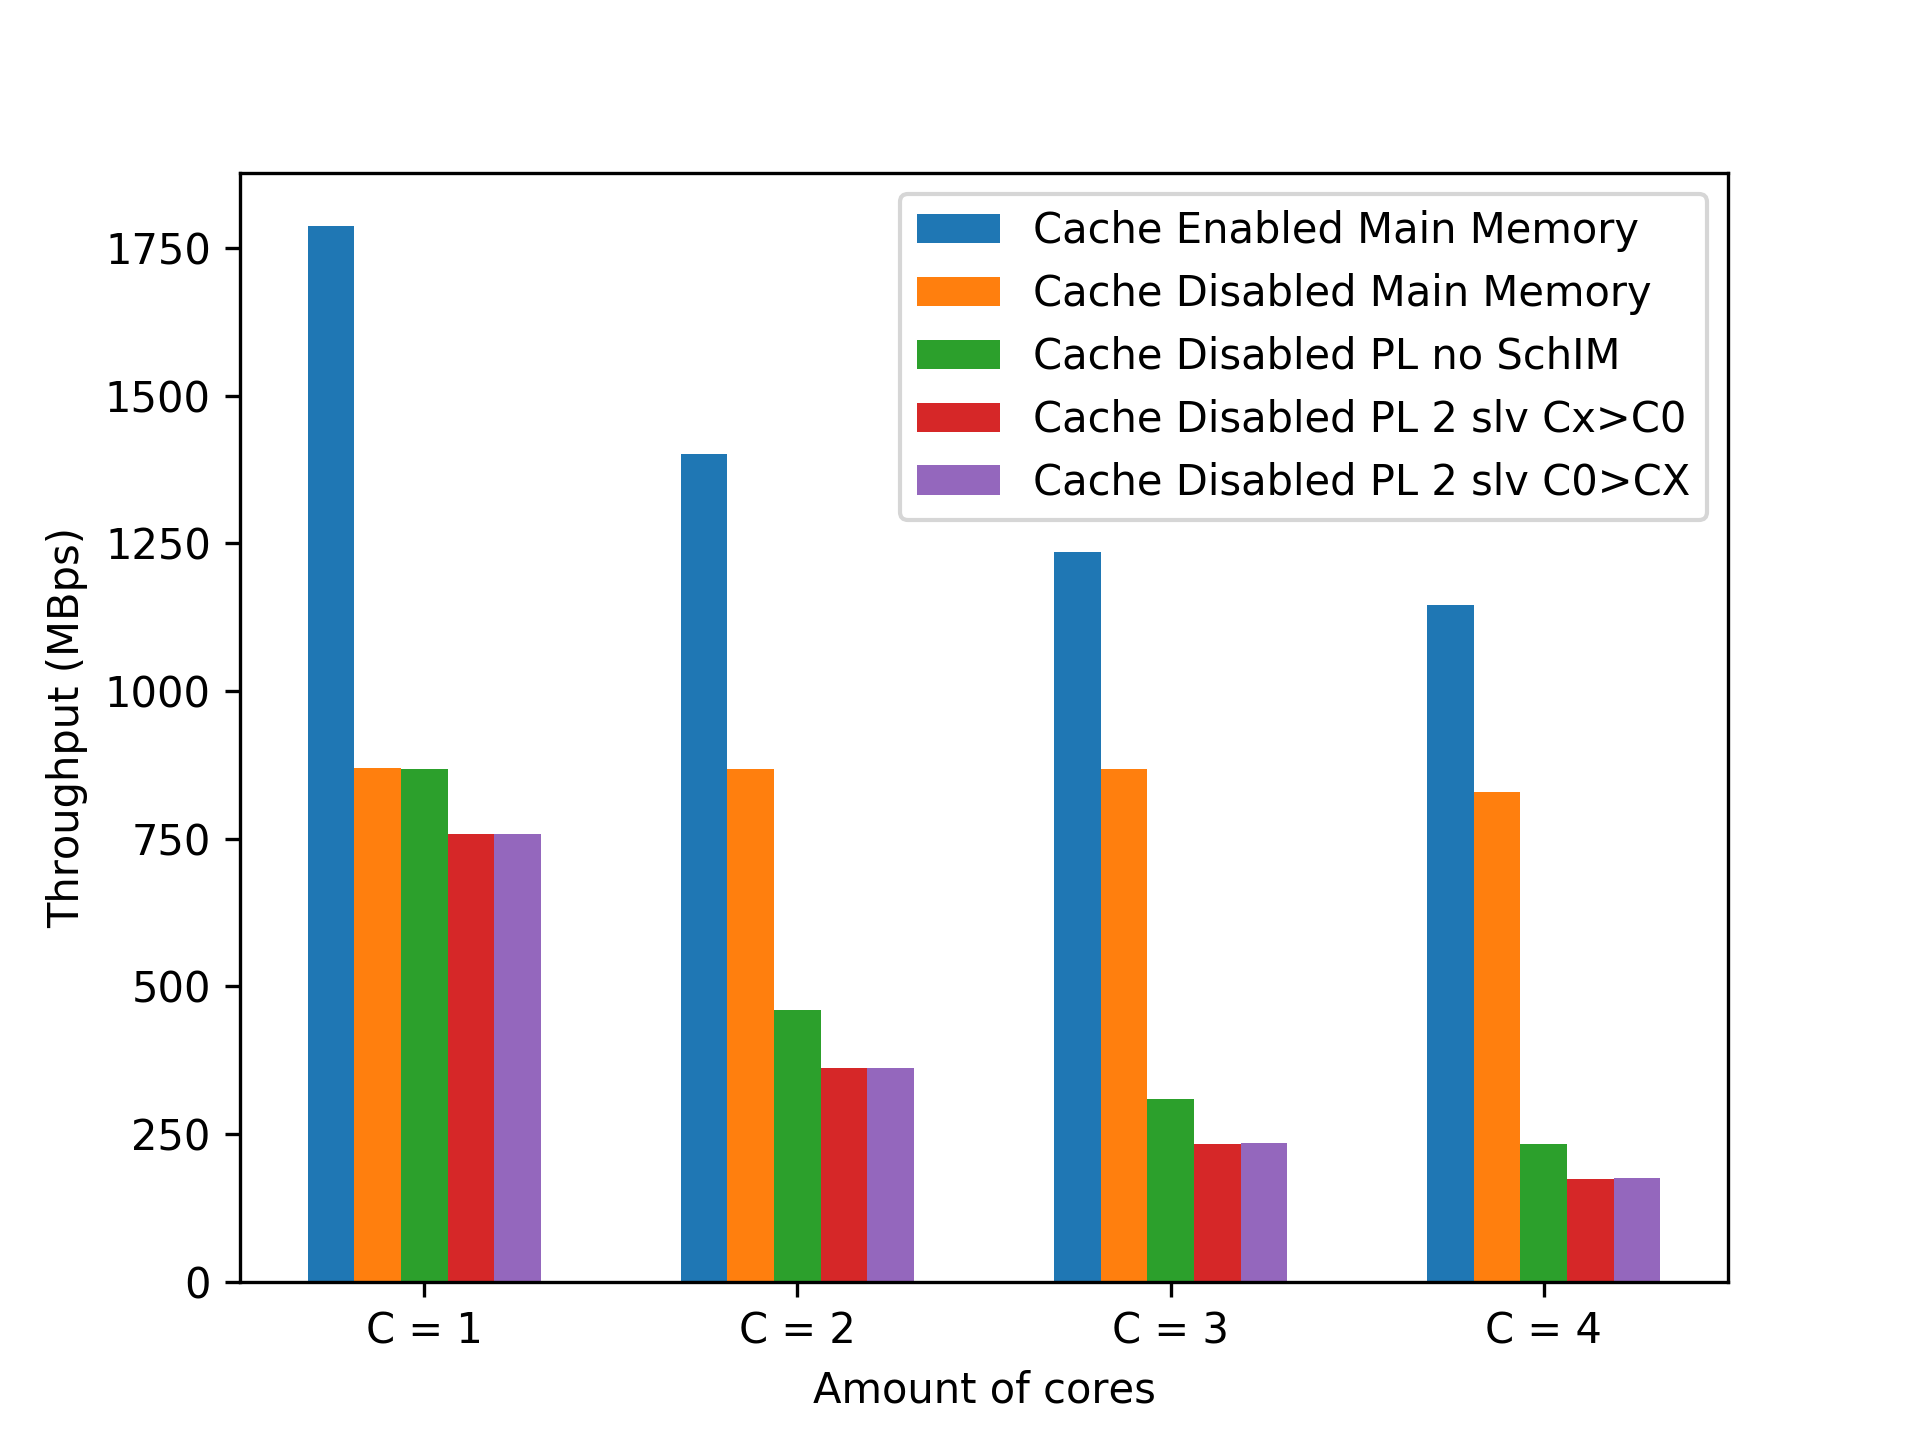
\includegraphics[scale=0.5]{../doc/experiments/bw_comparisons.png}
      \caption{Board bandwidth}
      \label{fig:bandwidth_comparison}
      \todo[inline]{TODO: outdated version. Has to be repeated for cached transactions only with the latest version of SchIM.}
    \end{figure}
    
  \subsection{Internal Behaviour of SchIM}
    Here, show and emphasize on the behaviour of SchIM with Fig.\ref{fig:schim_behaviour}
    \todo[inline]{Here, we use the trace snapshots}
    \begin{figure*}
      \begin{subfigure}{.3\textwidth}
        \centering
        % include first image
        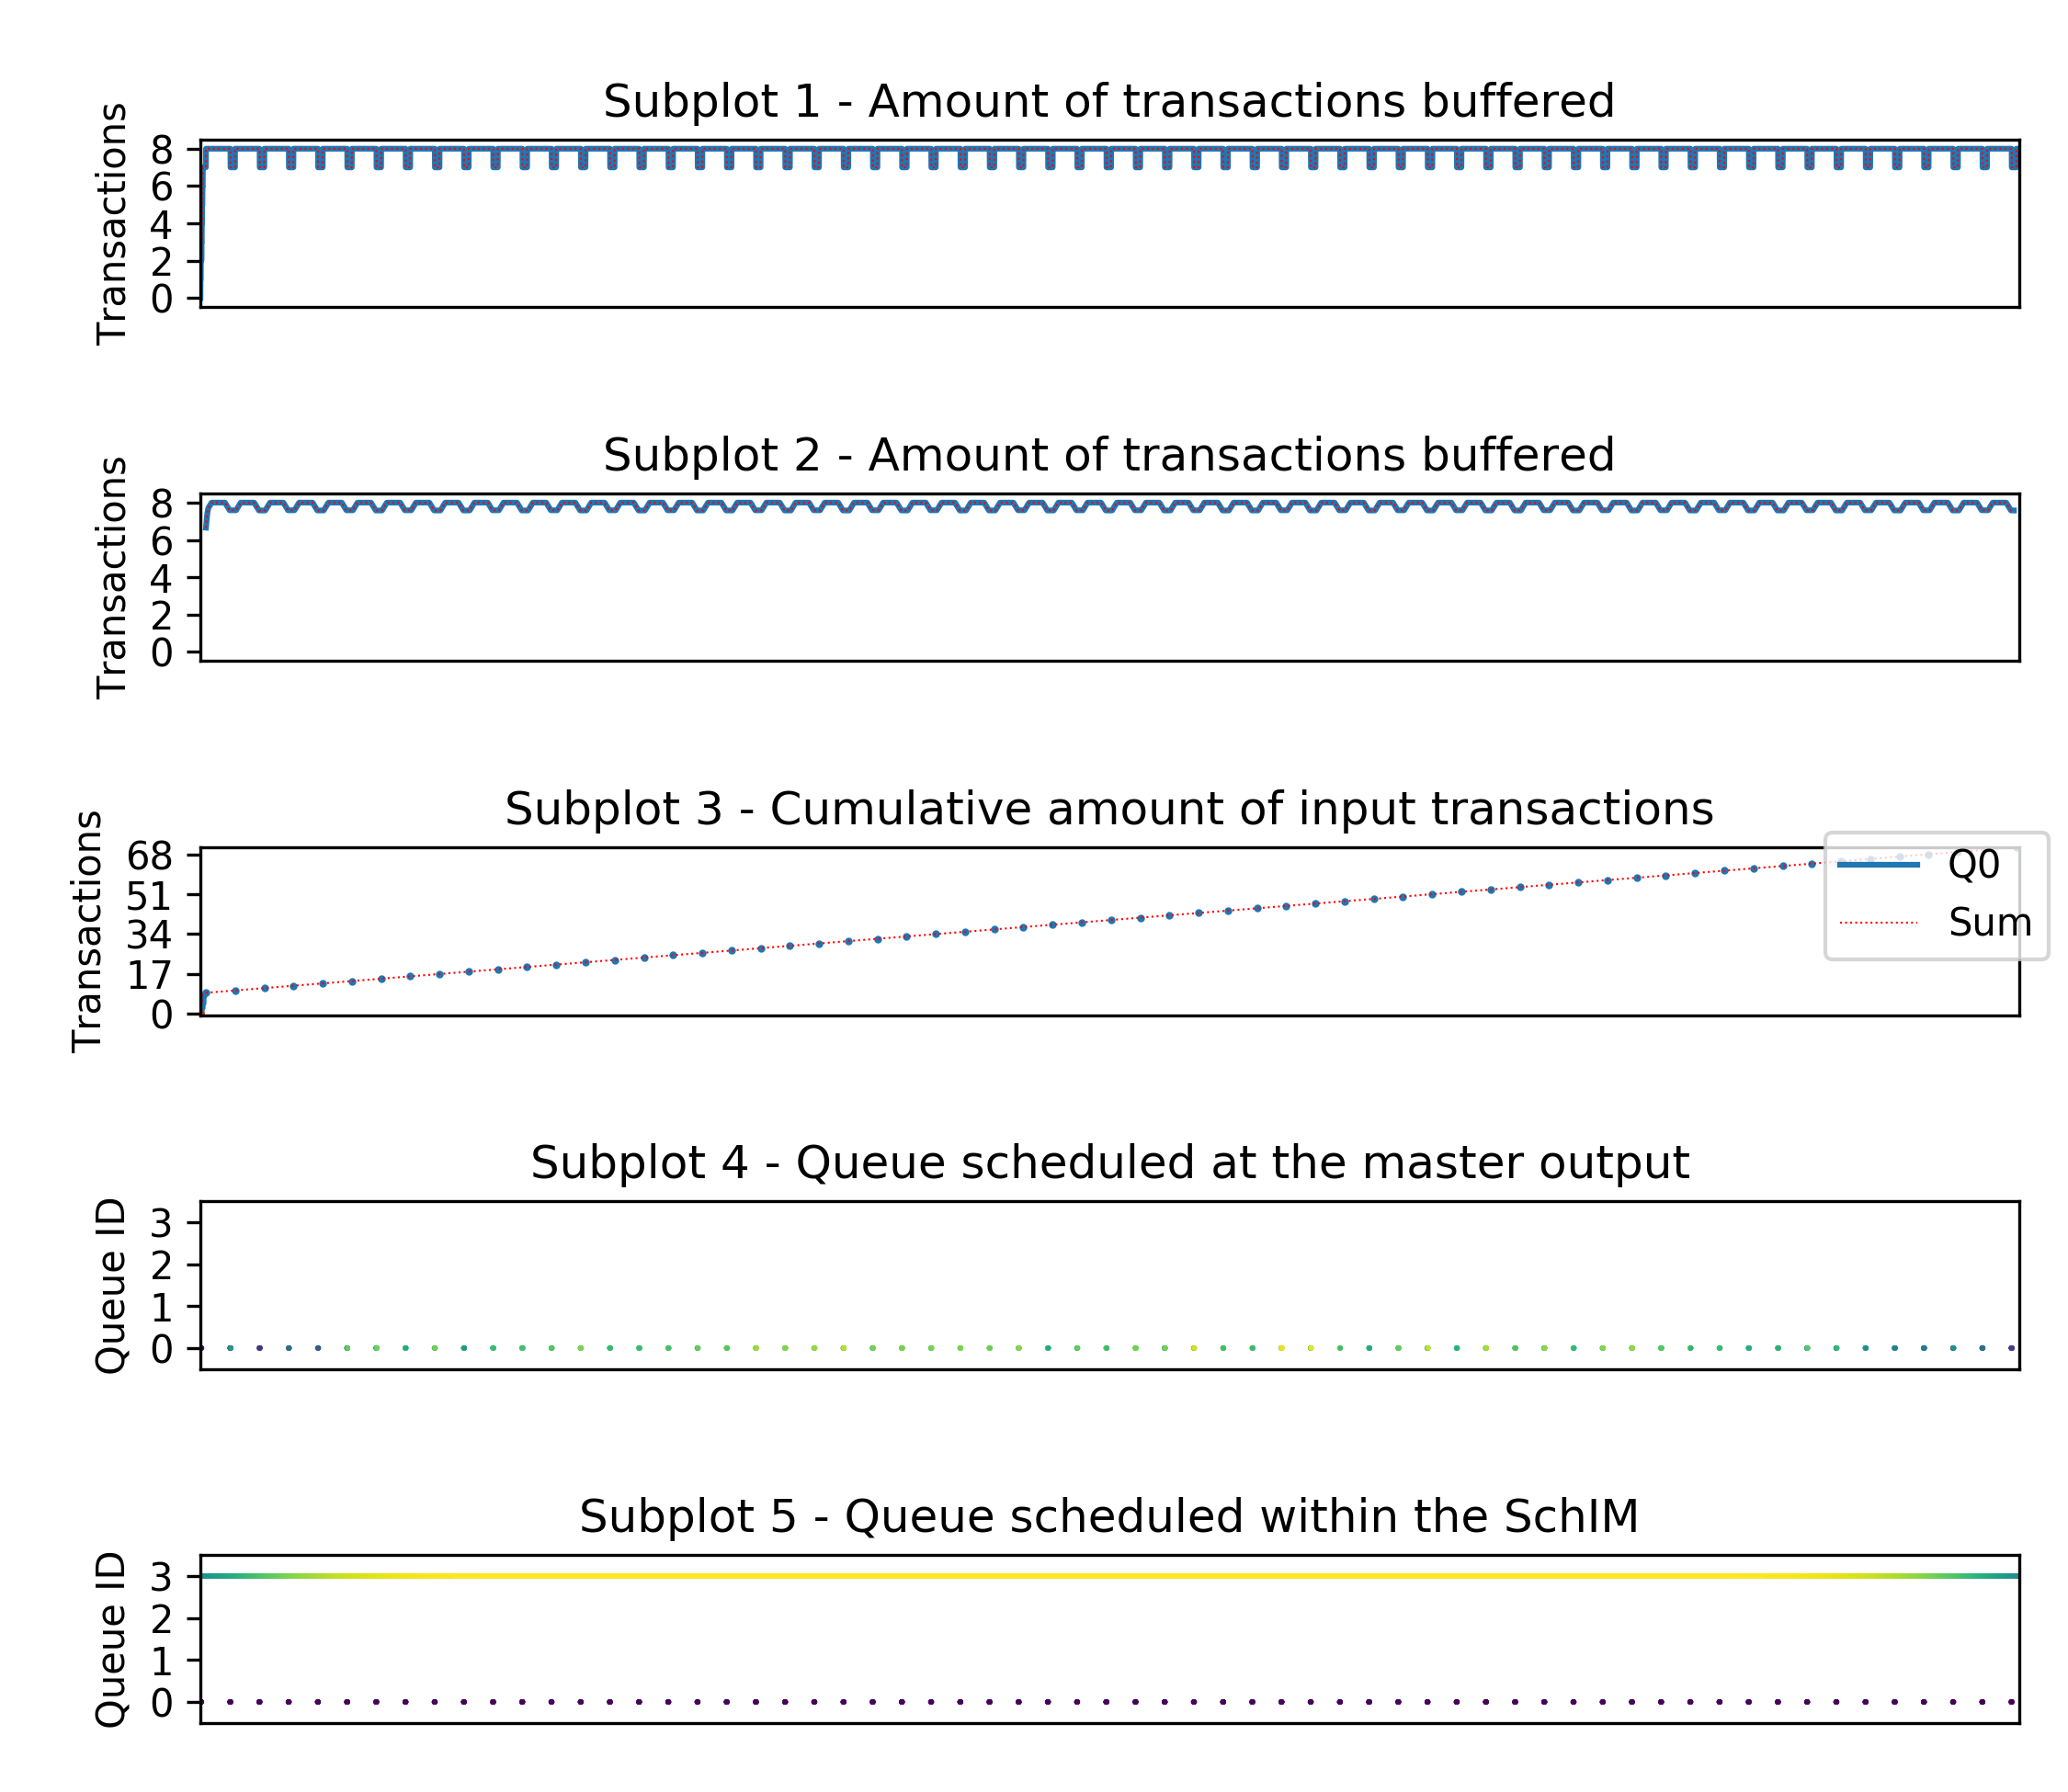
\includegraphics[scale=0.31]{../doc/experiments/buffering_4c_15_08_FP.png}  
        \caption{Put your sub-caption here}
        \label{fig:schim_behaviour_fp}
      \end{subfigure}
      \hfill
      \begin{subfigure}{.3\textwidth}
        \centering
        % include second image
        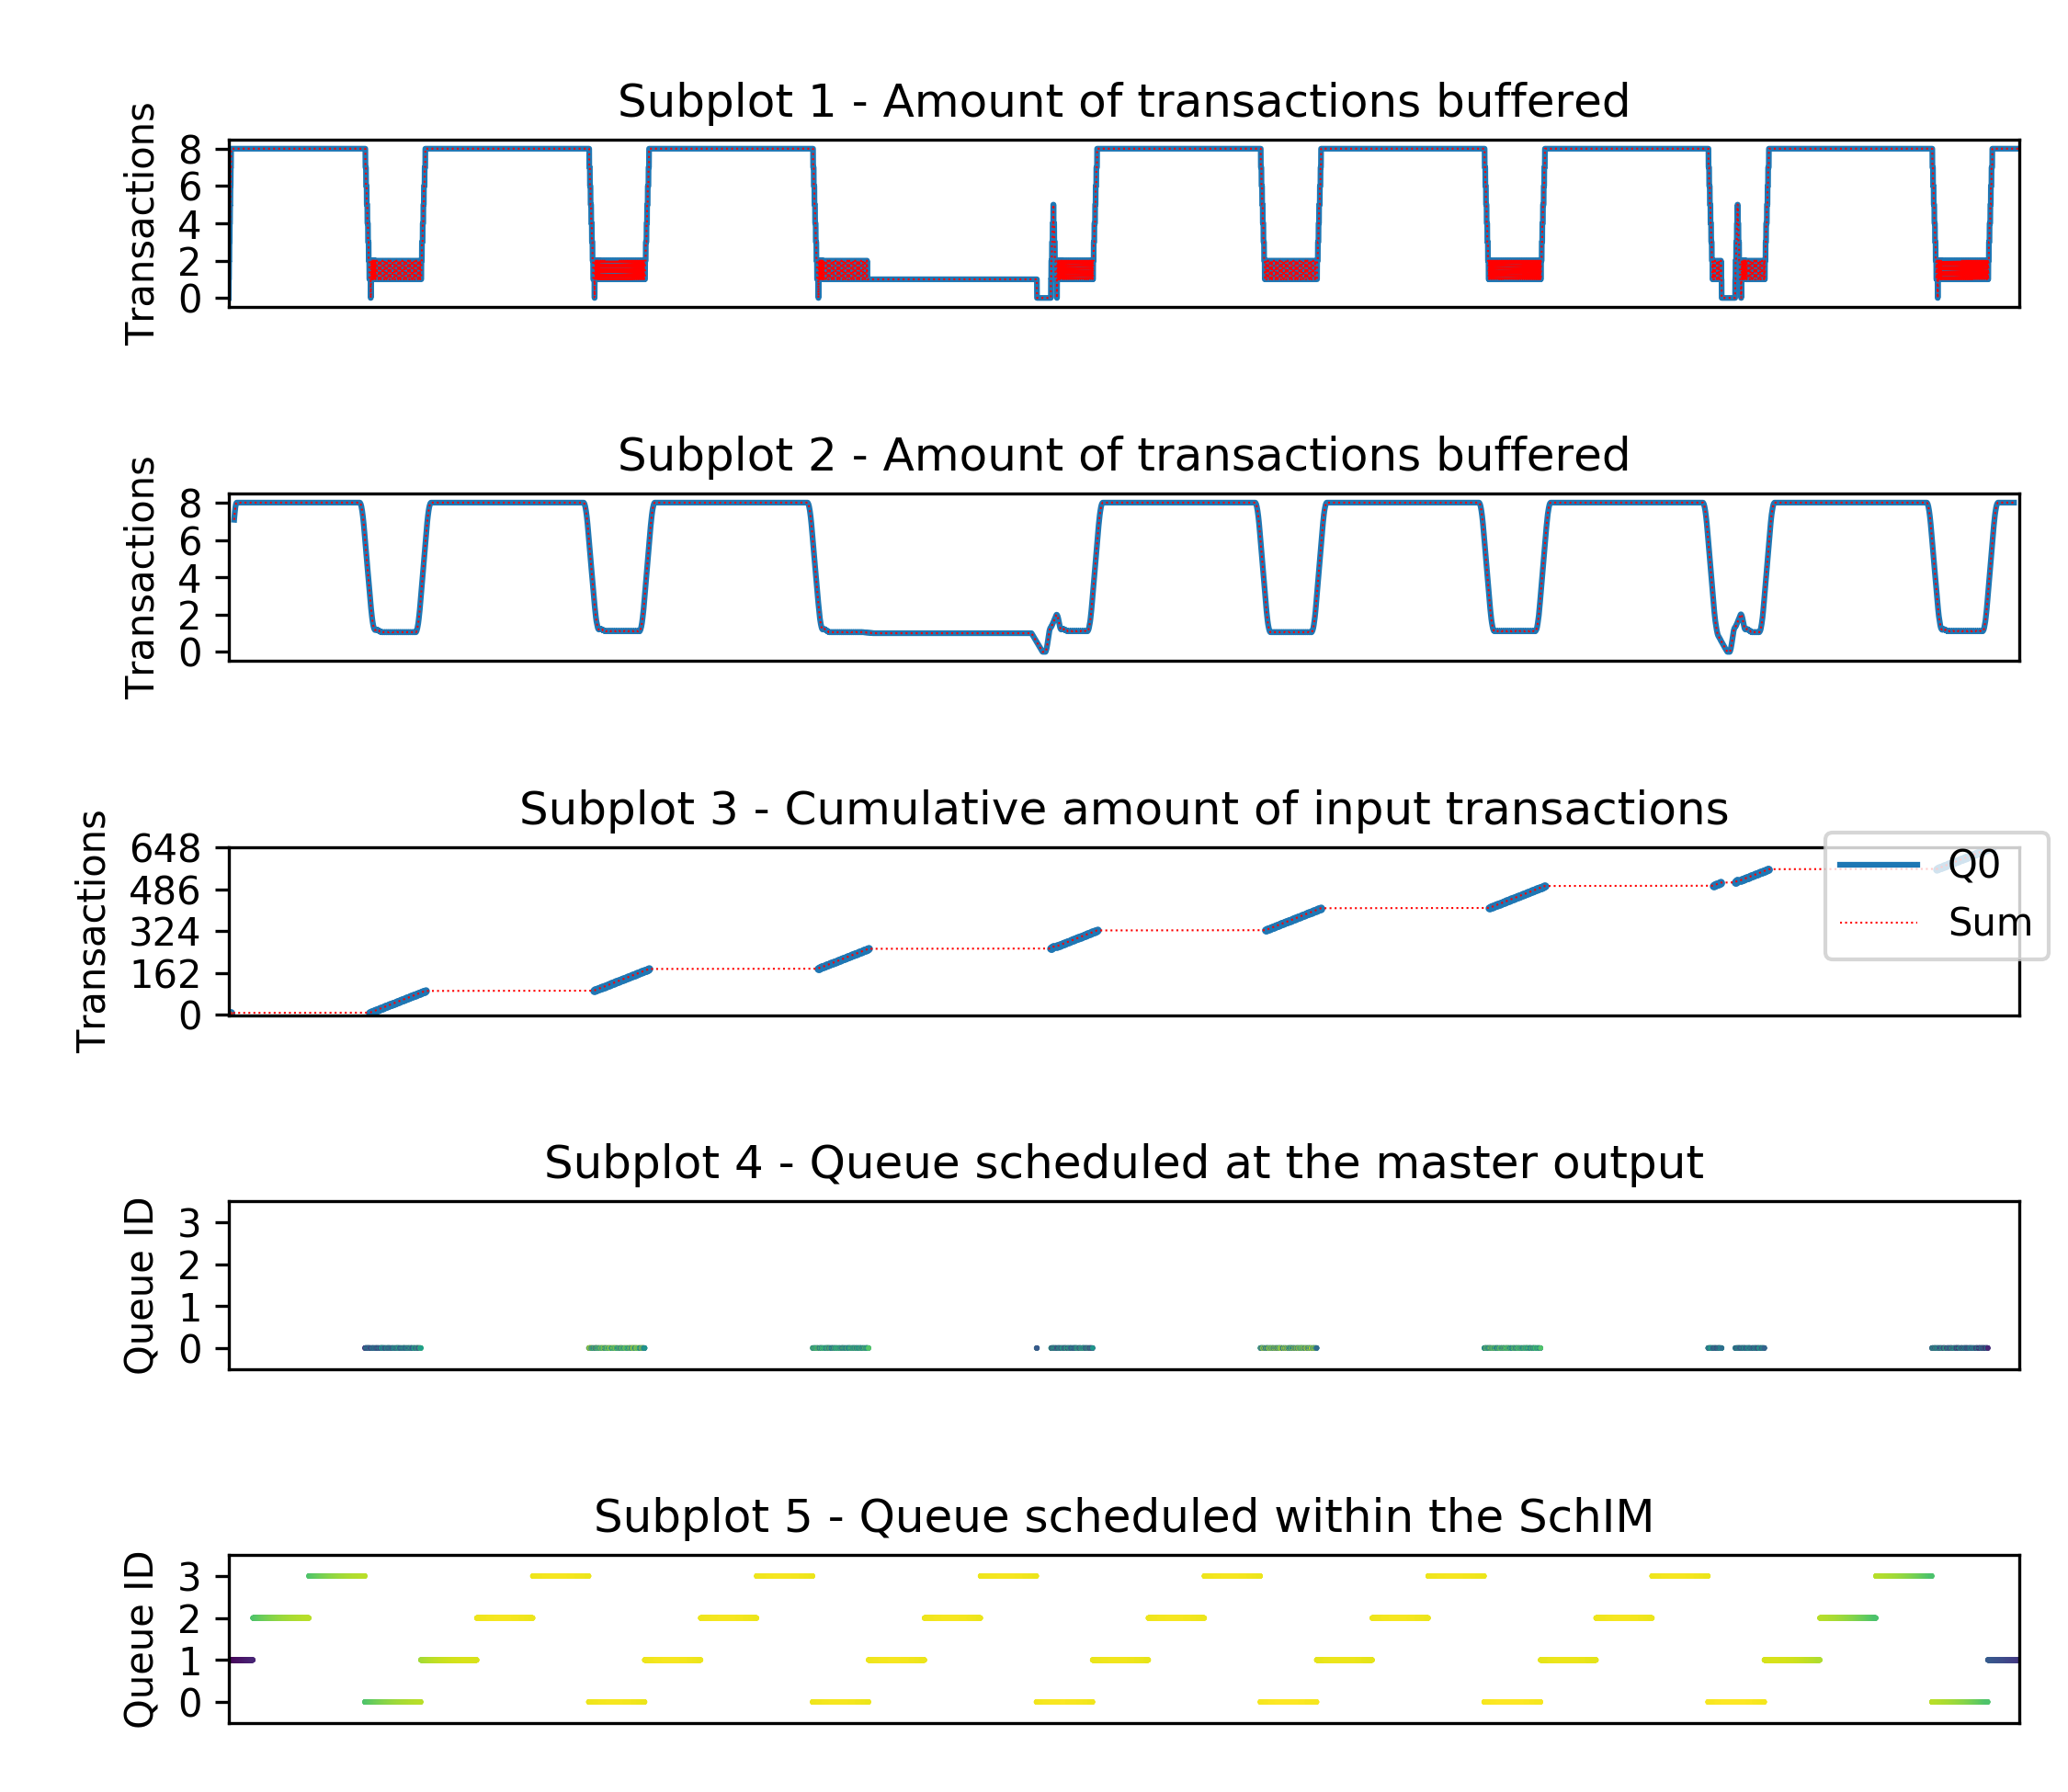
\includegraphics[scale=0.31]{../doc/experiments/buffering_4c_15_08_TDMA.png}  
        \caption{Put your sub-caption here}
        \label{fig:schim_behaviour_tdma}
      \end{subfigure}
      \hfill
      \begin{subfigure}{.3\textwidth}
        \centering
        % include second image
        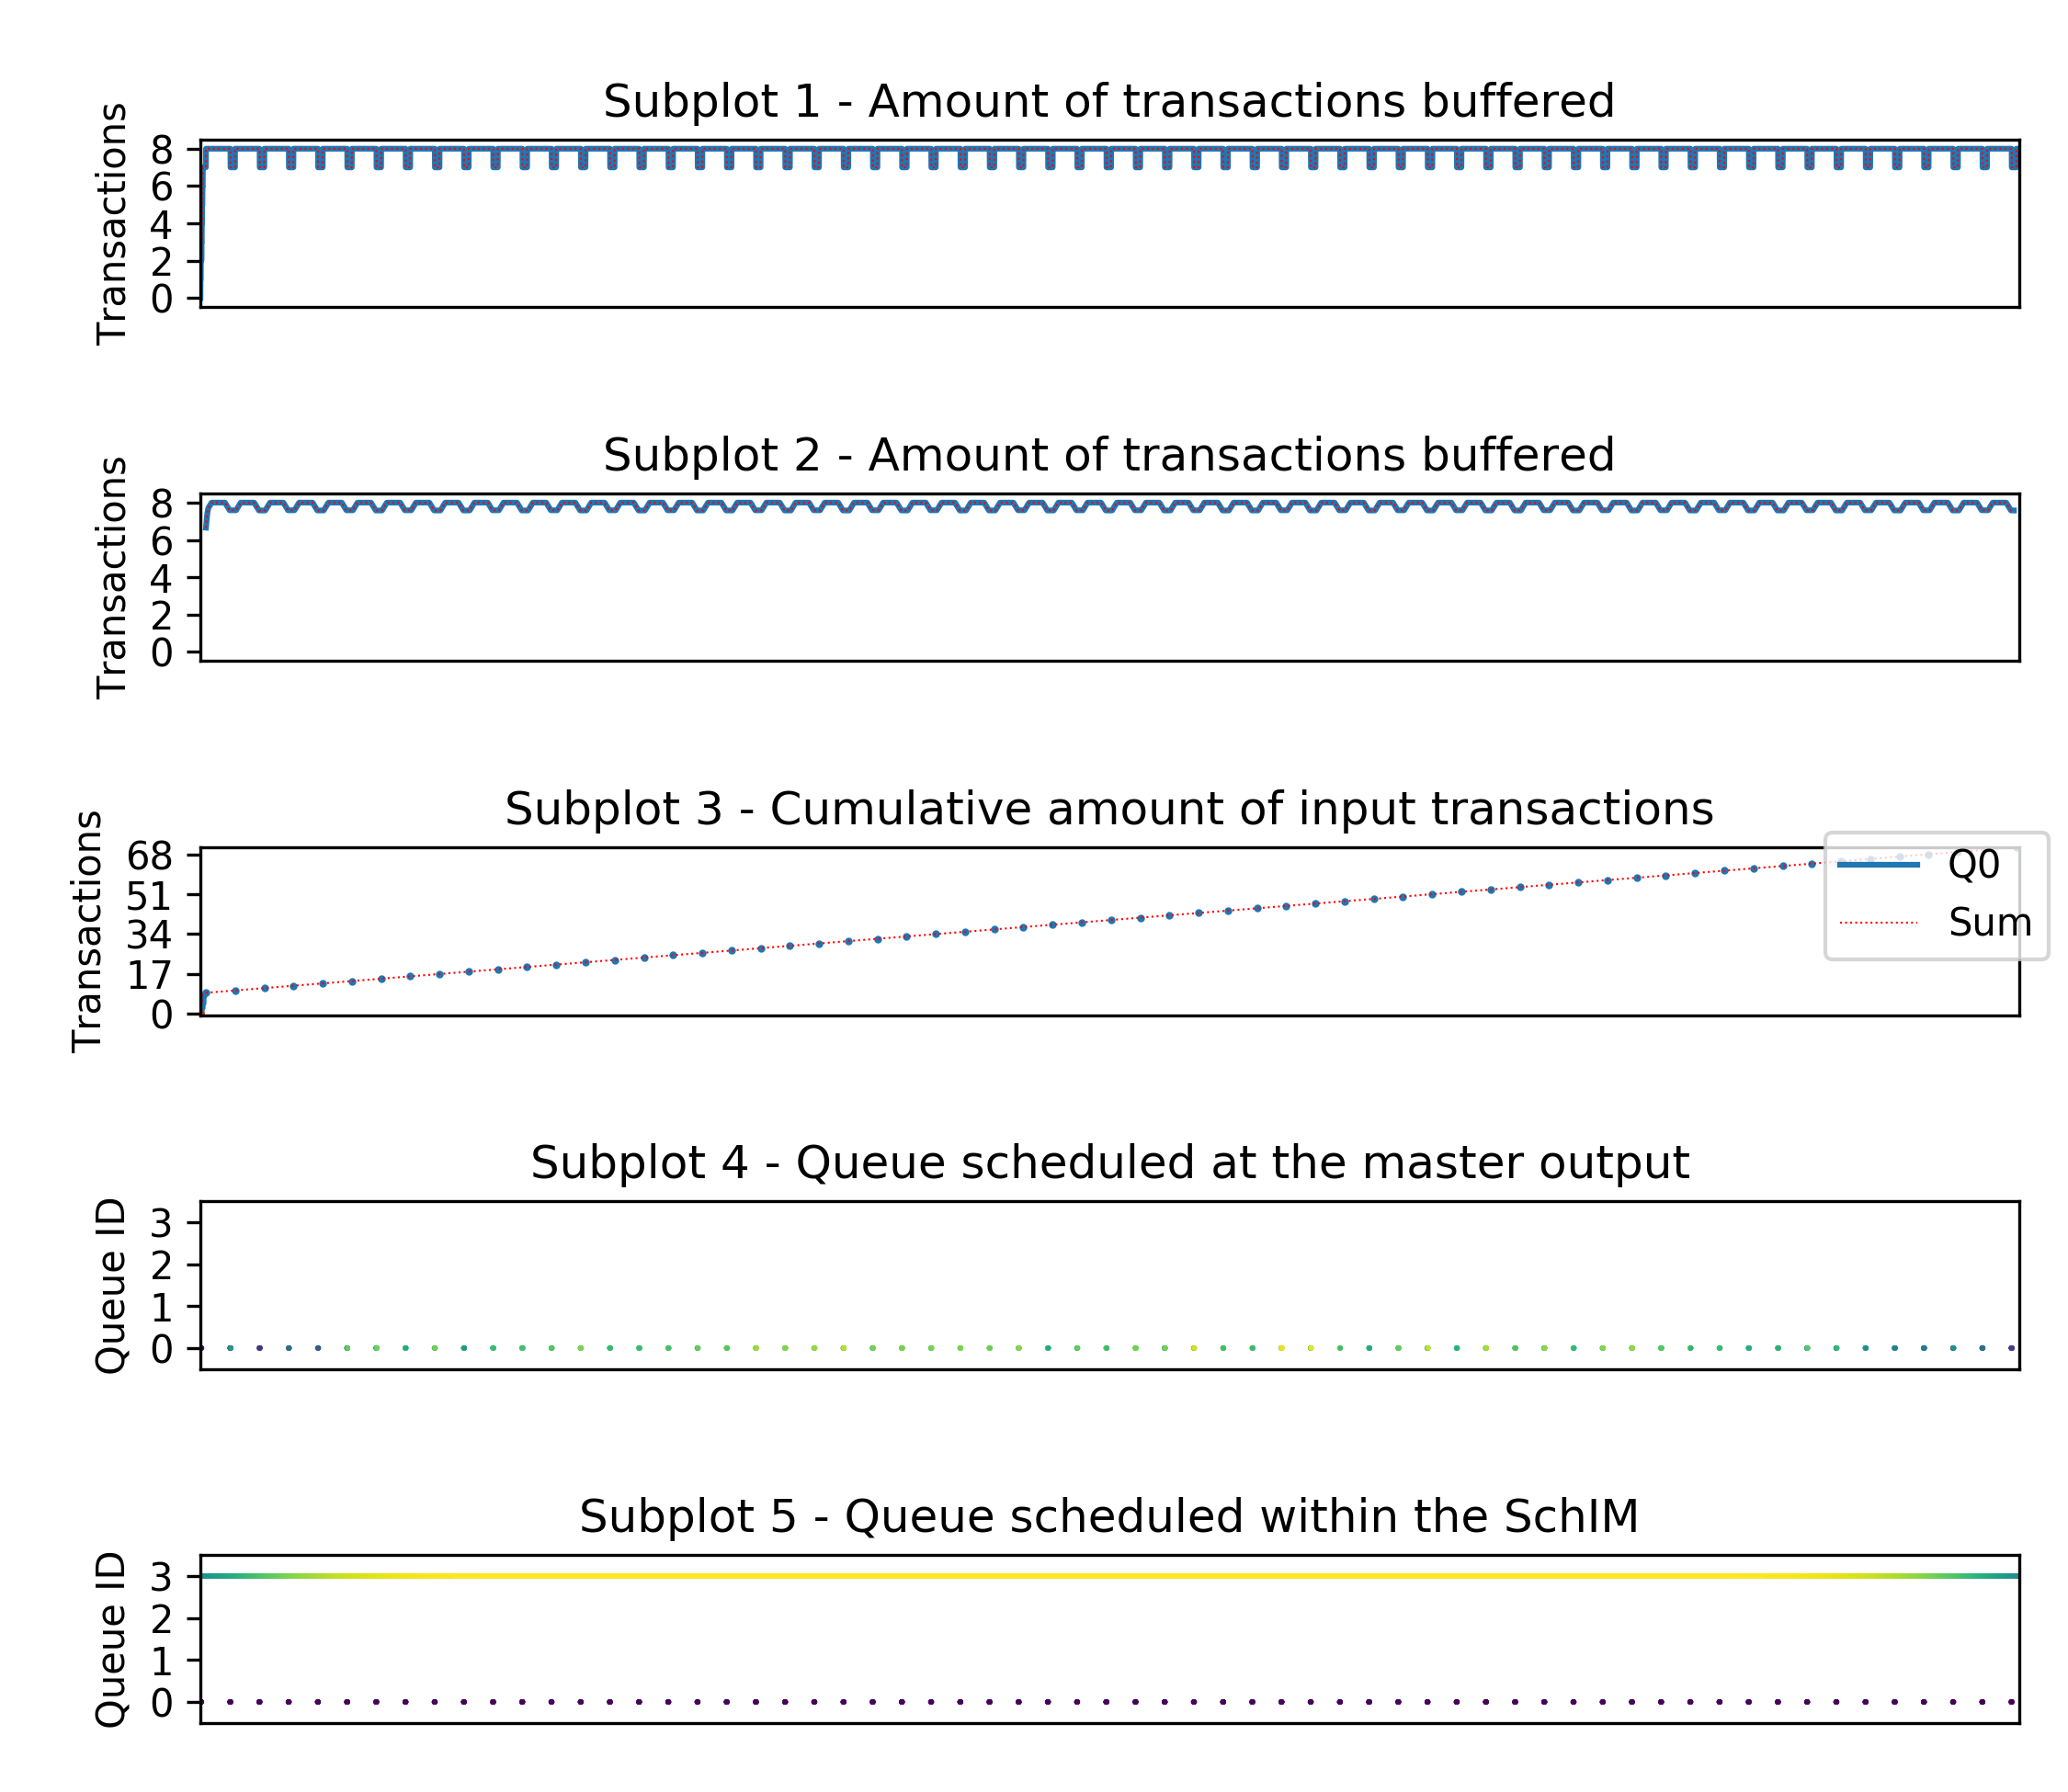
\includegraphics[scale=0.31]{../doc/experiments/buffering_4c_15_08_MG.png}  
        \caption{Put your sub-caption here}
        \label{fig:schim_behaviour_mg}
      \end{subfigure}
      \caption{Put your caption here}
      \label{fig:schim_behaviour}
      \todo[inline]{TODO: outdated version. Has to be repeated for cached transactions only with the latest version of SchIM and the plots have to be reworked.}
    \end{figure*}
    
  \subsection{Memory Isolation}
%    \todo[inline]{Here, prove that SchIM enables us to isolate the cores. We need a bunch of benchmarks competing with mem-bombs on the remaining cores. We will try:
    \begin{itemize}
      \item FP:~ The benchmark running alone with the highest priority VS. the same setup with mem-bombs
      \item TDMA:~ The benchmark running alone with all the cores having a slot of the same size VS. the same setup with mem-bombs
      \item MG:~ The benchmark running alone with all the cores having a given periodicity VS. the same setup with mem-bombs
    \end{itemize}
%    }
